\documentclass[conference]{IEEEtran}
\usepackage{cite}
\usepackage{amsmath,amssymb,amsfonts}
\usepackage{algorithmic}
\usepackage{graphicx}
\usepackage{textcomp}
\usepackage{xcolor}
\usepackage{array}
\usepackage{ragged2e}
\usepackage{multirow} % For multirows in tables
\usepackage{float} % Appending the [H] option forces the placement of a figure in the place it's in the code
\graphicspath{ {./lab_2_figures/} }
% Used for a left-aligned table cell with given width
\newcolumntype{P}[1]{>{\RaggedRight\hspace{0pt}}p{#1}}

% The following is for typesetting Verilog
\usepackage{xcolor}
\usepackage{listings}
\definecolor{vgreen}{RGB}{104,180,104}
\definecolor{vblue}{RGB}{49,49,255}
\definecolor{vorange}{RGB}{255,143,102}
\lstdefinestyle{verilog-style}{
    language=Verilog,
    basicstyle=\small\ttfamily,
    keywordstyle=\color{vblue},
    identifierstyle=\color{black},
    commentstyle=\color{vgreen},
    numbers=left,
    numberstyle=\tiny\color{black},
    numbersep=3pt,
    tabsize=4,
    moredelim=*[s][\colorIndex]{[}{]},
    literate=*{:}{:}1
}
\makeatletter
\newcommand*\@lbracket{[}
\newcommand*\@rbracket{]}
\newcommand*\@colon{:}
\newcommand*\colorIndex{%
    \edef\@temp{\the\lst@token}%
    \ifx\@temp\@lbracket \color{black}%
    \else\ifx\@temp\@rbracket \color{black}%
    \else\ifx\@temp\@colon \color{black}%
    \else \color{vorange}%
    \fi\fi\fi
}
\makeatother

\begin{document}

\title{Lab 2 Report --- Register Files and Datapath\\
\Large{Computer Design Laboratory ECE 3710}\\
\Large{Fall 2021}\\
\Large{The University of Utah}}

\author{\IEEEauthorblockN{Jacob Peterson}
\IEEEauthorblockA{\textit{Computer Engineering 2022}\\
\textit{University of Utah}\\
Salt Lake City, UT}
\and
\IEEEauthorblockN{Brady Hartog}
\IEEEauthorblockA{\textit{Computer Engineering 2022}\\
\textit{University of Utah}\\
Salt Lake City, UT}
\and
\IEEEauthorblockN{Isabella Gilman}
\IEEEauthorblockA{\textit{Computer Engineering 2023}\\
\textit{University of Utah}\\
Salt Lake City, UT}
\and
\IEEEauthorblockN{Nate Hansen}
\IEEEauthorblockA{\textit{Computer Engineering 2023}\\
\textit{University of Utah}\\
Salt Lake City, UT}
}

\maketitle

\begin{abstract}
This paper reports on the ALU design and synthesis along with the regfile design and datapath integration for the CompactRISC16 (CR16) processor. First, the Algorithmic Logic Unit (ALU) design and implementation is explored in detail including: port list of the ALU Verilog module, opcodes and their associated encodings, operation status flags and their associated encodings. Then, the regfile design and implementation is discussed thoroughly with the following highlights: behavioral design with a Verilog \verb|generate| block, function detail, port list, and block diagram. Additionally, the overall organization and implementation of the ALU, regfile, and the datapath between the two is discussed in detail. Finally, the synthesis statistics are reported (number of Look-up Tables (LUT), ALMs, FFs, BUFs used) and a timing analysis report is included.
\end{abstract}

\section{Introduction}
The ALU and regfile which this paper covers are critical to the design and implementation of the CR16 processor. In the completed processor, the data path they create will handle all instructions programmed into the machine. In this design, the regfile is responsible for temporarily remembering values that are currently in use, while the ALU handles all arithmetic done by the processor. By combining the two, we create datapath that is able to read values from the regfile, process the values in the ALU, then save the output back in the regfile. This pattern makes up the core functionality of our processor.

\section{The CR16 ALU}
The CR16 ALU implements the opcodes shown in Table \ref{table_alu_opcodes}. Our ALU implementation uses a large case block for the given opcode that executes behavioral operations for the respective operation. The following shows some arithmetic operations that our behavioral Verilog in our ALU uses:
\begin{itemize}
    \item \verb|+| is the addition operator which is used to add numbers in both signed and unsigned contexts with 2's complement numbers.
    \item \verb|-| is the subtraction operator which is used to add numbers in both signed and unsigned contexts with 2's complement numbers.
    \item \verb|>| and \verb|<| are numerical comparison operators which is used to set various status bits for a given operation.
    \item \verb|&|, \text{\textbar}, \verb|^|, and \verb|~| are boolean logic operators for AND, OR, XOR, and NOT respectively which are used for specific opcodes and in combinational logic for setting the flag bits on certain operations.
    \item \verb|<<| and \verb|>>| are logic shift operators which perform bit-shift operations on the given operands.
    \item \verb|<<<| and \verb|>>>| are arithmetic shift operators which perform sign-extending bit-shift operations on the given operands.
\end{itemize}
As seen in Table \ref{table_alu_opcodes}, there is no regard for immediate values since the ALU synthesizes as purely combinational logic that is not concerned with the immediate values since those are going to be decoded from a given processor instruction and passed to the ALU individually. The module signature containing the port list is seen in Figure \ref{figure_cr16_alu_module_signature}.

\begin{table} \centering
    \caption{ALU Opcodes}
    \label{table_alu_opcodes}
    \begin{tabular}{ | P{5em} | P{5em} | P{12em} | }
        \hline
        \textbf{ALU Opcode} & \textbf{Instruction Encoding} & \textbf{Description} \\
        \hline
        ADD & 0 & Signed addition \\
        \hline
        ADDU & 1 & Unsigned addition \\
        \hline
        ADDC & 2 & Signed addition with carry \\
        \hline
        ADDCU & 3 & Unsigned addition with carry \\
        \hline
        SUB & 4 & Signed subtraction \\
        \hline
        SUBU & 5 & Unsigned subtraction \\
        \hline
        AND & 6 & Bitwise AND \\
        \hline
        OR & 7 & Bitwise OR \\
        \hline
        XOR & 8 & Bitwise XOR \\
        \hline
        NOT & 9 & Bitwise NOT \\
        \hline
        LSH & 10 & Logical left shift \\
        \hline
        RSH & 11 & Logical right shift \\
        \hline
        ALSH & 12 & Arithmetic (sign-extending) left shift \\
        \hline
        ARSH & 13 & Arithmetic (sign-extending) right shift \\
        \hline
    \end{tabular}
\end{table}

\begin{table} \centering
    \caption{ALU Status Bit Mappings}
    \label{table_alu_status_bit_mappings}
    \begin{tabular}{ | P{5em} | P{5em} | P{12em} | }
        \hline
        \textbf{Status Bit} & \textbf{Status One-Hot Encoding} & \textbf{Description} \\
        \hline
        CARRY & \verb|5'b00001| & MSB carry out for unsigned addition and subtraction \\
        \hline
        LOW & \verb|5'b00010| & \verb|B < A| for unsigned subtraction \\
        \hline
        FLAG & \verb|5'b00100| & MSB carry out for signed addition \\
        \hline
        ZERO & \verb|5'b01000| & Set when \verb|C == 0| \\
        \hline
        NEGATIVE & \verb|5'b10000| & \verb|B < A| for signed addition and subtraction \\
        \hline
    \end{tabular}
\end{table}

\begin{figure}
    \begin{lstlisting}[style={verilog-style}]
module cr16_alu
      #(parameter integer P_WIDTH = 16)
       (input wire I_ENABLE,
        input wire [3 : 0] I_OPCODE,
        input wire [P_WIDTH - 1 : 0] I_A,
        input wire [P_WIDTH - 1 : 0] I_B,
        output reg [P_WIDTH - 1 : 0] O_C,
        output reg [4 : 0] O_STATUS);
    \end{lstlisting}
    \caption{The CR16 ALU module signature with port list.}
    \label{figure_cr16_alu_module_signature}
\end{figure}

\section{The CR16 Regfile}

The CR16 register file consists of 16 general-purpose, 16-bit registers. The block diagram is shown in Figure \ref{fig:regfile_block_diagram}.

\begin{figure}[htbp]
    \centering
    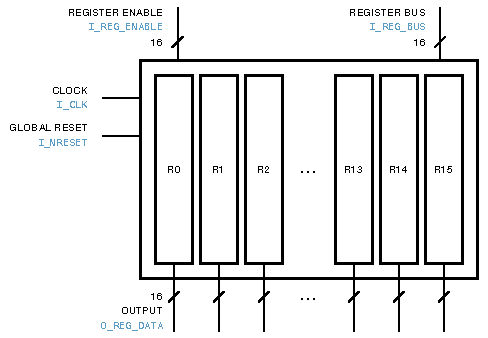
\includegraphics[scale=1.0]{lab_2_figures/regfile_block_diagram.pdf}
    \caption{Block diagram of the CR16 register file.}
    \label{fig:regfile_block_diagram}
\end{figure}

In our implementation, the register file module, \verb|cr16_regfile|, uses the \verb|parameter| construct to parameterize: 1) the bit width of the registers, and 2) the number of registers. These parameters are both 16 by default. The module has a global RESET control which is tied to every register; it has a multi-channel ENABLE control that can enable the registers individually. In practice, this ENABLE control enables only one register at a time, which is the register to be written on any given instruction. The value to be written is input via the register bus, which is connected from the output of the ALU to every register. The output of the register file is a vector of size (number of registers) × (bit width) of all data in the registers.

The output vector is connected to the read ports of the ALU. In keeping with modern convention, the read ports are designed as multiplexors rather than as tri-state buffers. For the register file, this means that, unlike with tri-state buffers, both read ports have one register selected at any given time. This design choice presents a challenge for instructions that wish to use the same register as both an operand and the result; such instructions cannot be executed in a single clock cycle, as this approach would require the register to be simultaneously read by a read port and written by the register bus. The solution to this challenge is the subject of future work.

\section{Datapath}
The datapath of the cr16 architecture is a union of the ALU to the register file. We made a few design decisions here to aid in incremental implementation and testing of the unit. The following is a block diagram detailing the top-level view of our datapath, including a dummy finite state machine with hard-coded instructions to aid in the testing and synthesis:

\subsection{Inputs}
The inputs of the datapath will be controlled later on by the CPU controller. They consist of the following:
\begin{enumerate}
    \item I\_NRESET: A global reset for the register file and flags register.
    \item I\_OPCODE: The opcode to be supplied to the ALU.
    \item I\_ENABLE: Global enable signal for ALU and read from all registers.
    \item I\_CLK: Clock signal for sequential logic in registers.
    \item I\_REG\_A\_SELECT/I\_REG\_B\_SELECT: Each of these are 4-bit selector signals designed to pass one register from each write port (A and B) to the next element on the datapath. We'll discuss this further when we elaborate on multiplexer implementation.
    \item I\_IMMEDIATE: 16-bit value to be supplied as an immediate if the instruction implements one.
    \item I\_IMMEDIATE\_SEL: Selector for the multiplexer that decides whether to allow an immediate value or the value from read port A to be active at the input A of the ALU.
\end{enumerate}

\subsection{Outputs}
The outputs are much more simple. They are mainly used for testing and will likely be removed when SRAM and CPU control are implemented:
\begin{enumerate}
    \item O\_RESULT\_BUS: The bus that connects the output of the ALU to the write port of the register file. This output is necessary to properly test the functionality of the datapath.
    \item O\_STATUS\_FLAGS: The bus that connects the ALU flags output to the write port of the flags register. This output is necessary to ensure flags are reported and written correctly.
\end{enumerate}

We decided to implement multiplexer-based control flow since that is used most commonly in modern CPU architectures. Selector signals are supplied to the read ports A and B, and to the multiplexer array at ALU input A which decides whether to pass the Regfile read port A or the immediate value supplied to the datapath.

\subsection{Read Port Multiplexing}
The multiplexer logic at read ports A and B is quite extensive. The register file gives access to a 2-dimensional array containing all the data stored in each of the registers. To consolidate this to two selected ports, we first implemented a model for a 16-to-1 multiplexer. This multiplexer consists of a 16-bit input, a 1-bit output, and a 4-bit selector as shown in Fig. \ref{fig:16_to_1_mux}.

\begin{figure}[htbp]
    \centering
    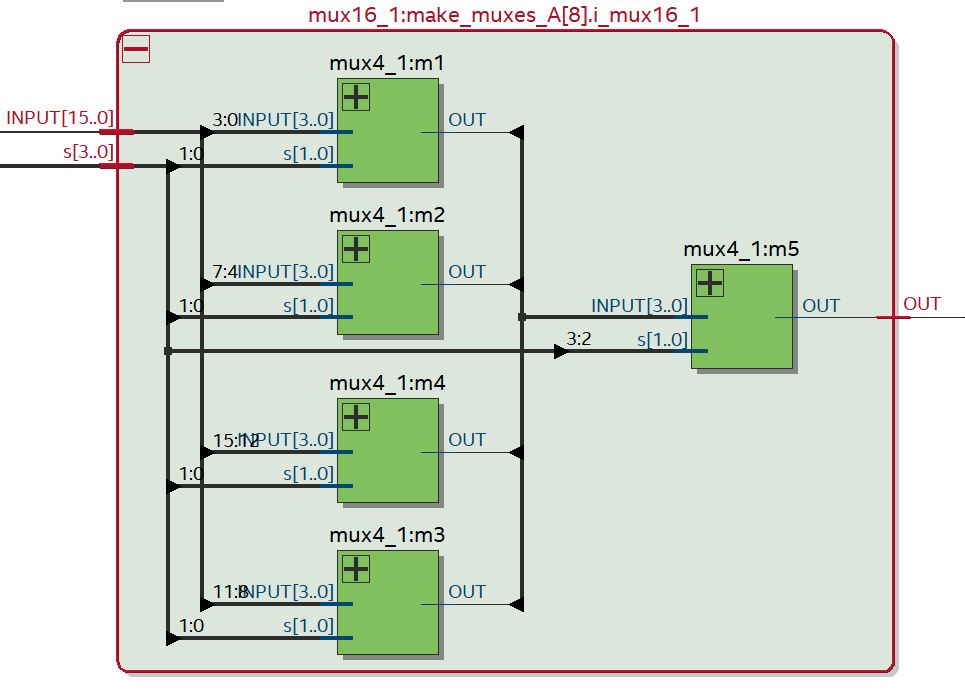
\includegraphics[scale=0.3]{lab_2_figures/16-to-1-mux.JPG}
    \caption{16-to-1 Multiplexer with 4-bit selector as seen in Quartus RTL viewer.}
    \label{fig:16_to_1_mux}
\end{figure}
To establish one read port, we instantiate 16 of these 16-to-1 multiplexers and connect each one to the nth bit of every register. For example, the first 16-to-1 mux is connected to the LSB of each r0-r15. This allows us to feed the same 4-bit selector to each mux and draw out a 16-bit vector consisting of the data from one of the registers in the Regfile. We specify \textit{which} register by setting the selector signal to the decimal value 0-15 corresponding to the desired register. The connections appear as shown in Fig. \ref{fig:read_port_mux_connections}.

\begin{figure}[h]
    \centering
    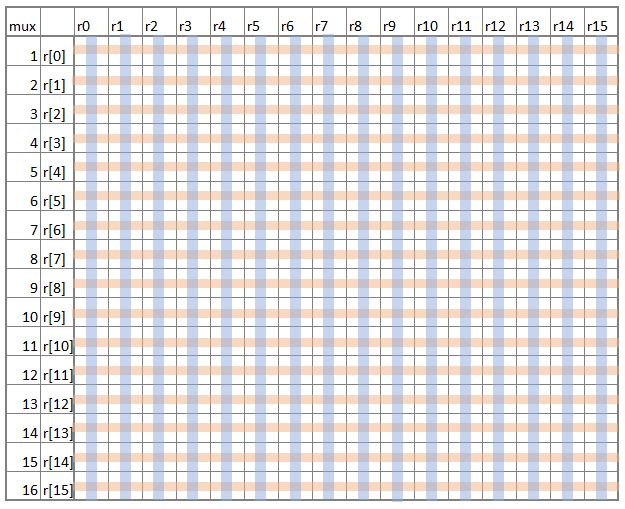
\includegraphics[scale=0.50]{lab_2_figures/read_port_mux_connections.JPG}
    \caption{Read Port to 16x16-to-1 Mux Connections}
    \label{fig:read_port_mux_connections}
\end{figure}

\subsection{Immediate Value Multiplexing}
To control the use of immediate values, we can use a vector of 2-to-1 multiplexers--essentially a 32-to-16 mux--to select either the immediate supplied to the datapath or the value from read port A. Each mux is supplied the same 1-bit selector signal from the CPU control. This prevents conflicts on bus A. A diagram of this implementation is shown in the full block diagram in Fig. \ref{fig:datapath_block_diagram}.

\begin{figure}[h]
    \centering
    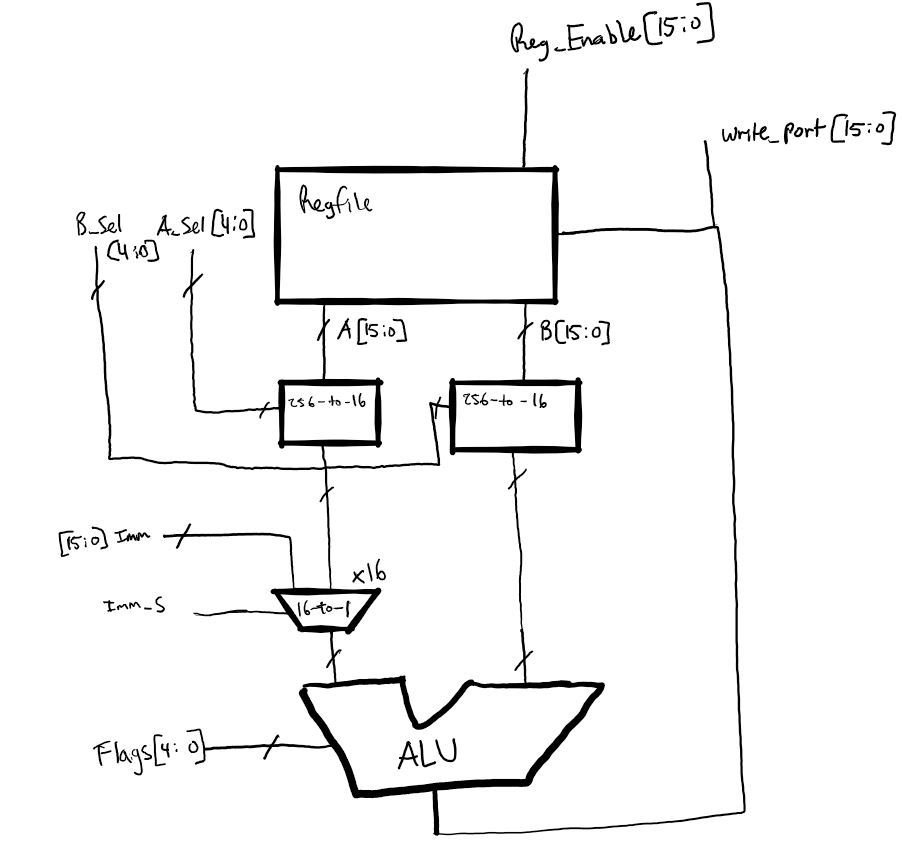
\includegraphics[scale=0.45]{lab_2_figures/block_diagram_datapath.JPG}
    \caption{Block diagram for datapath. Global enables and resets omitted for graphic clarity.}
    \label{fig:datapath_block_diagram}
\end{figure}

This datapath will synthesize sequential logic, and therefore it is easiest to test it for correct functionality using a Finite State Machine.

\section{Testing with Testbenches and the FSM}
We conducted testing in two ways: by simulating a dummy set of instructions in a testbench, and by hard-coding some CPU control into a simple FSM to synthesize with the datapath and display outputs on the FPGA.
\subsection{The Testbench}
The testbench we have written consists of four separate tests designed to exercise multiple unique functions of the datapath.
\begin{enumerate}
    \item Test 1 simulates 15 iterations of the Fibonacci Sequence by writing a 1 into r0 and r1, then writing each subsequent answer into a subsequent register through r15.
    \item Test 2 loads a 0 value into all 16 registers and then attempts to subtract 1 from register r1 to show signed arithmetic is possible.
    \item Test 3 loads 0111 into r1 and 0100 into r2. Various logical Boolean operations are conducted on these values to determine the correct function of logical operations.
    \item Test 4 loads integer 1 into registers r1 and r2. The test then attempts and writes a total of 15 sequential bit-shifts on registers r1-r15 to ensure proper functionality of the shift operation.
\end{enumerate}

The first three tests in the testbench show working functionality of the datapath, while the fourth is a work-in-progress.

\subsection{The FSM Hardware Test}
We have hard-coded an FSM program using case statements that will execute 7 stages of the Fibonacci sequence and populate the first 8 registers of the register file. The demonstration of this functionality is available to view at https://youtu.be/-uqqciOsI4k.

The demo shows the use of a single FPGA button as a global reset. We also use a button from the FPGA to simulate the advancement of each state in the FSM program. This button is tied to the clock cycle so that the datapath and Regfile respond to the changes in the input values each time that the state advances. This is a simple demonstration that will extend into larger functionality as we move forward to the implementation to the full FSM of the CPU control.

\section{Synthesis Reports and Timing Analysis}
We reviewed the synthesis reports of the datapath module independent of the FSM and top-level module we used for hardware testing. The following data was obtained.
\subsection{Synthesis Reports}
\begin{figure}[h]
    \centering
    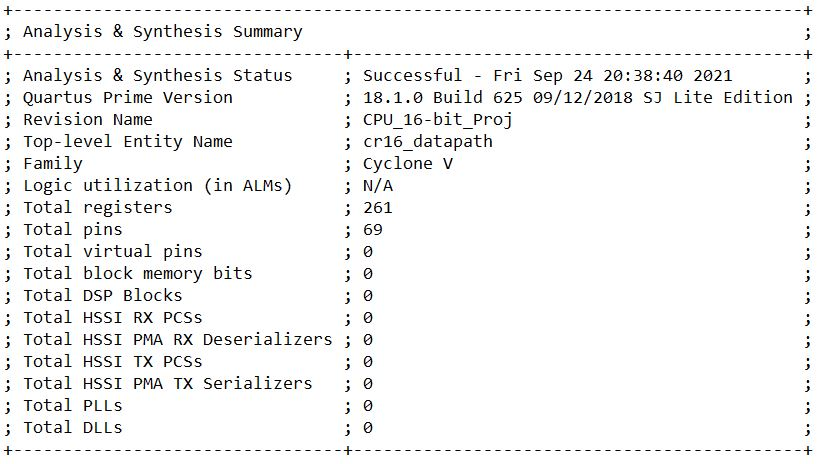
\includegraphics[scale=0.5]{lab_2_figures/analysis_and_synthesis_summary.JPG}
    \caption{Summary data from the Quartus map synthesis report after synthesizing "cr16\_datapath.v" as the top-level module.}
    \label{fig:datapath_analysis_summary}
\end{figure}

As is shown in the summary of the synthesis report (Fig. \ref{fig:datapath_analysis_summary}), the datapath occupies 261 total registers and contains 69 pins. This is substantial. It is likely that the logic surrounding the multiplexing of the regfile's read ports is occupying memory. Our code is functional in nature, so Quartus will make decisions behind the scenes that we cannot control regarding the synthesis of multiplexer logic. This is made even more apparent from the perspective of the netlist and resource occupation, which can be seen in Fig. \ref{fig:datapath_analysis_netlist} and Fig. \ref{fig:datapath_analysis_resources}. There is a high volume of fanout on each 16-bit bus that has to propagate signals through 16 inputs of a mux, and our design utilizes a total of 32 16-to-1 multiplexers. The implementation of these muxes is carried out hierarchically beginning from the level of a 2-to-1 mux, so the resulting logic circuit will contain many levels of hierarchical multiplexing. This increases the LUT depth significantly. The synthesis report details the average LUT depth at 8.82, while the maximum LUT depth is 10. This is considerable, but understandable considering our design strategy. This could be avoided in multiple ways. Perhaps there is a more efficient design strategy that would allow us to use less hardware to properly multiplex the read ports of the register file while still taking advantage of the portability of multiplexers. Further, we considered implementing the control of data reading using tri-state buffers. We were advised not to do this in the specification, but we believe it would decrease the hardware complexity and reduce LUT depth.

\begin{figure}[h]
    \centering
    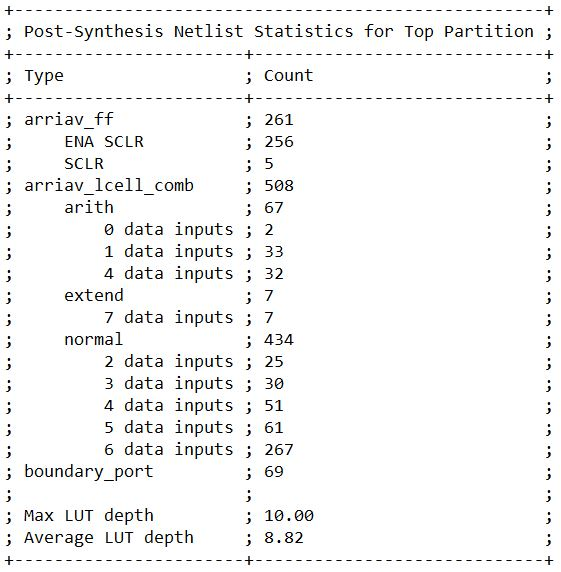
\includegraphics[scale=0.5]{lab_2_figures/analysis_and_synthesis_netlist.JPG}
    \caption{Netlist data from the Quartus map synthesis report after synthesizing "cr16\_datapath.v" as the top-level module.}
    \label{fig:datapath_analysis_netlist}
\end{figure}

Considering the average fan-out of our design is also a crucial element of efficiency analysis. While we do not have any other implementations of this particular piece of hardware to which we could compare our design, it is instructive to review the data. Total fan-out in our implementation is reported to be 3653, which is considerable. Average fan-out for each net is 4.08. The maximum fanout node is the global reset input, which is connected to each register in the Regfile and the flags register. The fanout of this node is so high (277) because each 16-bit register is likely synthesized using an array of 1-bit flip-flops. This means that the I\_NRESET signal will be connected to 16 flip-flops * 16 registers, or about 256 ports. The other 21 connections exist within the Regfile and the flags register. Other fanout occurs like this among connections like I\_ENABLE that have to be connected to many single-bit elements of the low level hardware synthesis.
\begin{figure}[h]
    \centering
    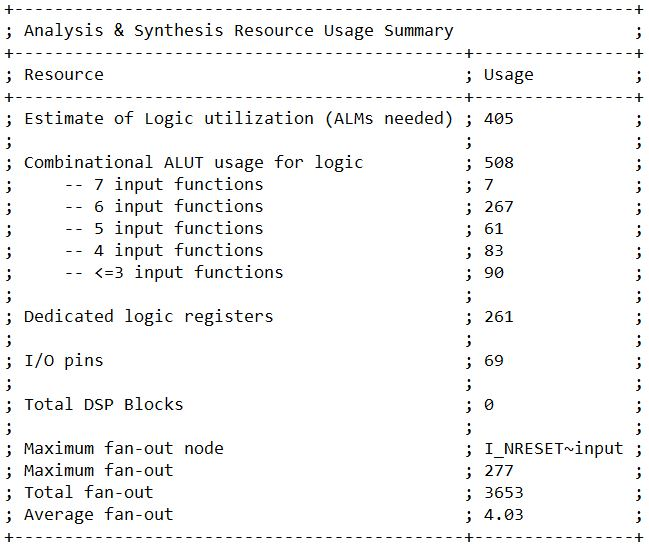
\includegraphics[scale=0.5]{lab_2_figures/analysis_and_synthesis_resources.JPG}
    \caption{Resource data from the Quartus map synthesis report after synthesizing "cr16\_datapath.v" as the top-level module.}
    \label{fig:datapath_analysis_resources}
\end{figure}
Overall it's hard to claim that our design is more or less efficient than others. It occupies comparatively few of the 85k available Logic Elements, so there are no constraints that would force us to rework our implementation for lack of resources.

\subsection{Timing Analysis}
We conducted timing analysis using the Quartus Timing Analyzer tool. This analysis contains the maximum time delay data from the input ports to the output ports of the datapath module, independent of the testing FSM and top-level module. We have included the top 25 longest propagation paths in Fig. \ref{fig:datapath_timing_table}.
\begin{figure}[h]
    \centering
    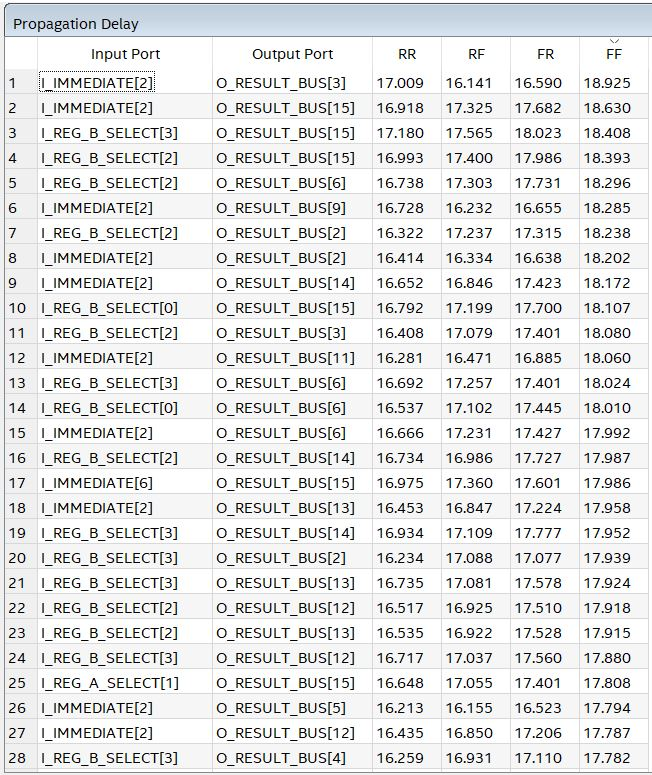
\includegraphics[scale=0.6]{lab_2_figures/timing_analysis_datapath.JPG}
    \caption{Timing analysis of top 25 maximum propagation times along the datapath from all inputs to all outputs.}
    \label{fig:datapath_timing_table}
\end{figure}
Regarding both Rise-Rise and Fall-Fall time delays, it is apparent that the longest propagation times occur along the signal path from the read port selectors to the write port along the result bus. This makes sense since there are 4 levels of multiplexing occurring in the read ports, and the signal propagation is delayed in that hierarchy. Since the register values are not seen as primary inputs, they will not appear in this analysis, but they have essentially the same critical path through each level of the multiplexer tree.
It is interesting to note that there doesn't seem to be a measurable difference between the propagation time of the MSB of selector B and the LSB of selector B. We would expect the selector bit connected to the top level of muxes to take longer to propagate than the bit connected to the final stage, but this is not the case. It is also not obvious why the selector signal for read port A propagates faster than that of read port B, since both seem to have symmetrical critical paths.
The signal providing an immediate value to the datapath also seems to show long propagation delays. Since it is only sent through one level of multiplexers to the ALU, we would expect it to propagate faster than the selector signals. It would seem to have a shorter critical path. However, the timing analyzer shows that the propagation of immediate values is more delayed than we expected. All of these delay times rest at or near 18ns-19ns. This will likely be too great a delay to utilize the kinds of clocks that modern processors can use, but perhaps a slower clock like the ones on the FPGA will not run too fast for our implementation.

\section{Conclusion}
The datapath implementation we have built is subject to modification as the project progresses and we better understand the overall functionality of the CR16 CPU. We have yet to implement a proper system that will load immediate values into the Regfile. The opcode mapping will likely look different from the perspective of the CPU control and FSM, so when we implement instruction decoding we will have two separate instruction encodings that will belong to the ALU and the CPU respectively. The CPU will have to interpret instructions exactly as they are decoded from the ISA, and this will allow the CPU to handle immediate instructions separately and control this behavior within the datapath and Regfile. We intend to clarify these details as we move forward so we can integrate a better version of this datapath/ALU module into our final working implementation of a CR16 CPU.
\end{document}
